%%%%%%%%%%%%%%%%%%%%%%%%%%%%%%%%%%%%%%%%%%%%%%%%%%%%%%%%%%%%%%%%%%%%%%
% writeLaTeX Example: A quick guide to LaTeX
%
% Source: Dave Richeson (divisbyzero.com), Dickinson College
% 
% A one-size-fits-all LaTeX cheat sheet. Kept to two pages, so it 
% can be printed (double-sided) on one piece of paper
% 
% Feel free to distribute this example, but please keep the referral
% to divisbyzero.com
% 
%%%%%%%%%%%%%%%%%%%%%%%%%%%%%%%%%%%%%%%%%%%%%%%%%%%%%%%%%%%%%%%%%%%%%%
% How to use writeLaTeX: 
%
% You edit the source code here on the left, and the preview on the
% right shows you the result within a few seconds.
%
% Bookmark this page and share the URL with your co-authors. They can
% edit at the same time!
%
% You can upload figures, bibliographies, custom classes and
% styles using the files menu.
%
% If you're new to LaTeX, the wikibook is a great place to start:
% http://en.wikibooks.org/wiki/LaTeX
%
%%%%%%%%%%%%%%%%%%%%%%%%%%%%%%%%%%%%%%%%%%%%%%%%%%%%%%%%%%%%%%%%%%%%%%

\documentclass[10pt,landscape]{article}
\usepackage{amssymb,amsmath,amsthm,amsfonts}
\usepackage{multicol,multirow}
\usepackage{enumitem}
\usepackage{calc}
\usepackage{ifthen}
\usepackage[landscape]{geometry}
\usepackage{graphicx, graphics, float}
\usepackage{caption}
\usepackage{longtable}

\usepackage[colorlinks=true,citecolor=blue,linkcolor=blue]{hyperref}
\usepackage{pdfpages}

\ifthenelse{\lengthtest { \paperwidth = 11in}}
    { \geometry{top=.5in,left=.5in,right=.5in,bottom=.5in} }
	{\ifthenelse{ \lengthtest{ \paperwidth = 297mm}}
		{\geometry{top=1cm,left=1cm,right=1cm,bottom=1cm} }
		{\geometry{top=1cm,left=1cm,right=1cm,bottom=1cm} }
	}
\pagestyle{empty}
\makeatletter
\renewcommand{\section}{\@startsection{section}{1}{0mm}%
                                {-1ex plus -.5ex minus -.2ex}%
                                {0.5ex plus .2ex}%x
                                {\normalfont\large\bfseries}}
\renewcommand{\subsection}{\@startsection{subsection}{2}{0mm}%
                                {-1explus -.5ex minus -.2ex}%
                                {0.5ex plus .2ex}%
                                {\normalfont\normalsize\bfseries}}
\renewcommand{\subsubsection}{\@startsection{subsubsection}{3}{0mm}%
                                {-1ex plus -.5ex minus -.2ex}%
                                {1ex plus .2ex}%
                                {\normalfont\small\bfseries}}
                                
\newcommand\todo[1]{\textcolor{red}{#1}}

\makeatother
\setcounter{secnumdepth}{0}
\setlength{\parindent}{0pt}
\setlength{\parskip}{0pt plus 0.5ex}

\theoremstyle{definition}
\newtheorem*{question}{Question}
\newtheorem*{defin}{Definition}

\theoremstyle{remark}
\newtheorem*{method}{Method}
\newtheorem*{remark}{Remark}


% -----------------------------------------------------------------------

\title{ELEC 202 Cheatsheet}

\begin{document}

\raggedright
\footnotesize

\begin{center}
     \Large{\textbf{ ELEC 202 Cheatsheet with \LaTeX}} \\
\end{center}

\begin{multicols}{3}
\setlength{\premulticols}{1pt}
\setlength{\postmulticols}{1pt}
\setlength{\multicolsep}{1pt}
\setlength{\columnsep}{2pt}

%%%%%%%%%%%%%%%%%%%%%%%%%%%%%%%%%%%%%%%%%%%%%%%%%%%%%%%%%%%%%
% Formating guides
%%%%%%%%%%%%%%%%%%%%%%%%%%%%%%%%%%%%%%%%%%%%%%%%%%%%%%%%%%%%%
% for no space list, use 
% [noitemsep,nolistsep]
% . It ony works for itemsize.
%%%%%%%%%%%%%%%%%%%%%%%%%%%%%%%%%%%%%%%%%%%%%%%%%%%%%%%%%%%%%
% FOr figures, use this:
% \begin{figure}[H]
%     \centering
%     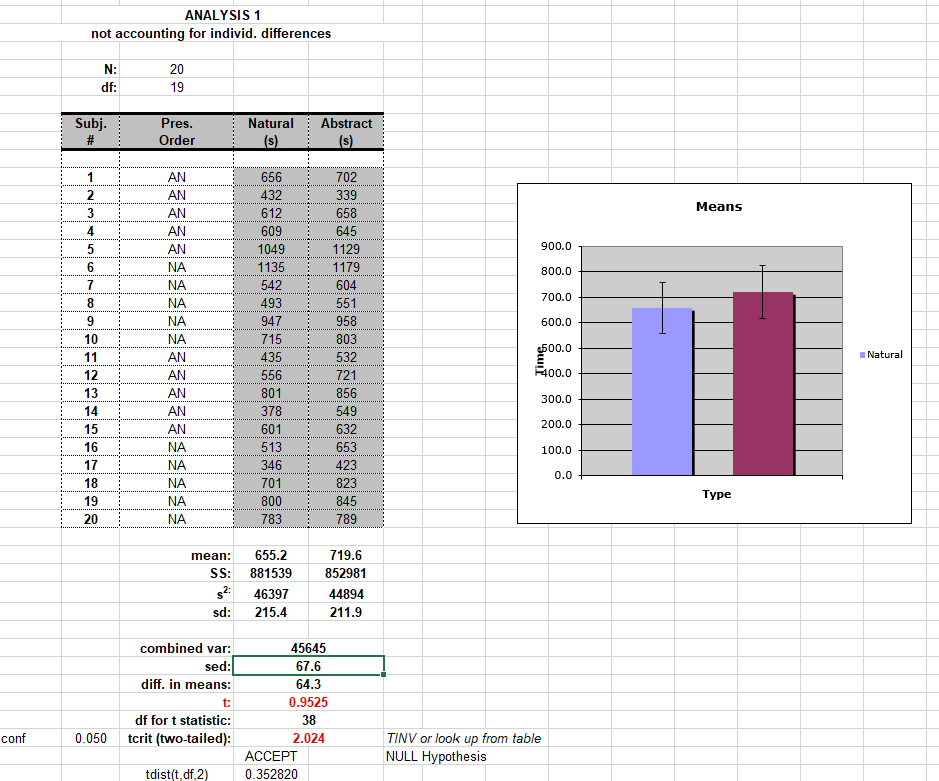
\includegraphics[width=\linewidth]{t-test.png}
%     \caption{Caption}
%     \label{fig:my_label}
% \end{figure}
%%%%%%%%%%%%%%%%%%%%%%%%%%%%%%%%%%%%%%%%%%%%%%%%%%%%%%%%%%%%%


%%%%%%%%%%%%%%%%%%%%%%%%%%%%%%%%%%%%%%%%%%%%%%%%%%%%%%%%%%%%%
% for no space list, use [noitemsep,nolistsep]. It ony works for itemsize.

%%%%%%%%%%%%%%%%%%%%%%%%%%%%%%%%%%%%%%%%%%%%%%%%%%%%%%%%%%%%%
%%%%%%%%%%%%%%%%%%%%%%%%%% section %%%%%%%%%%%%%%%%%%%%%%%%%%
%%%%%%%%%%%%%%%%%%%%%%%%%%%%%%%%%%%%%%%%%%%%%%%%%%%%%%%%%%%%%
\begin{remark}
Conventions: \\
\begin{itemize}[noitemsep,nolistsep]
    \item UPPER CASE symbols (I, V, Z) are in phasor domain. 
    \item Yes, $\imath$ is imaginary and i is current. imaginary $\imath$ are usually at MSB end of the equations. 
    \item all good looking images are from \cite{Alexander:2006:FEC:1207036}
    \item turn off independent source is replace voltage source with $v = 0$, which is a short circuit, and current source with open source. 
\end{itemize}
\end{remark}




%%%%%%%%%%%%%%%%%%%%%%%%%%%%%%%%%%%%%%%%%%%%%%%%%%%%%%%%%%%%%
%%%%%%%%%%%%%%%%%%%%%%%%%% section %%%%%%%%%%%%%%%%%%%%%%%%%%
%%%%%%%%%%%%%%%%%%%%%%%%%%%%%%%%%%%%%%%%%%%%%%%%%%%%%%%%%%%%%
\section{Basic Circuit}

\subsection{Terminology}
\begin{itemize}[noitemsep,nolistsep]
    \item Resistance: R = $\Re(Z) \; \Omega$
    \item Reactance: X = $\Im(Z) \; \Omega$
    \item Impedance: Z = $R + \imath X \; \Omega$
    \item Admittance: Y = $\frac{1}{Z} = G + \imath B \; S $
    \item Conductance: G = $\Re(\frac{1}{Z}) \; S$
    \item Susceptance: B = $\Im(\frac{1}{Z})\; S$
\end{itemize}



\subsection{Operational Amplifier}
\textbf{Ideal Op Amp}: 
\begin{figure}[H]
    \centering
    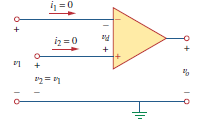
\includegraphics[width=0.5\linewidth]{202/figure/opamp.png}
    \caption*{Ideal Opamp}
    \label{fig:ideal_opamp}
\end{figure}

\begin{itemize}[noitemsep,nolistsep]
\item $i_1 = i_2 = 0$
\item $v_1 = v_2$
\end{itemize}

\textbf{Inverting Op Amp}:
\begin{figure}[H]
    \centering
    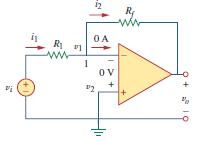
\includegraphics[width=0.5\linewidth]{202/figure/invert_opam.png}
    \caption{Inverting opamp}
    \label{fig:ideal_opamp}
\end{figure}
\begin{itemize}[noitemsep,nolistsep]
\item $v_0 = -\frac{R_f}{R_1}v_i$ 
\end{itemize}


\textbf{AC steady state}: frequency and amplitude are not varying and all current, voltage are at the same frequency(for phasor). If not, use circuit's superposition. \\
\textbf{DC steady state}: i and v of the circuit stopped changing. \\


%%%%%%%%%%%%%%%%%%%%%%%%%%%%%%%%%%%%%%%%%%%%%%%%%%%%%%%%%%%%%
%%%%%%%%%%%%%%%%%%%%%%%%%% section %%%%%%%%%%%%%%%%%%%%%%%%%%
%%%%%%%%%%%%%%%%%%%%%%%%%%%%%%%%%%%%%%%%%%%%%%%%%%%%%%%%%%%%%
\section{Analysis and Transformation}
\subsection{Laplace Transformation}
\begin{defin} \mbox{} \\
$s = \sigma + \imath\omega$ \\
Laplace: $\mathcal{L}$[f(t)] = F(s) = $\int^\infty_{0^-}f(t)e^{-st}dt$ \\
Inverse Laplace: $\mathcal{L}^{-1}$[F(s)] = f(t) = $\frac{1}{2\pi \imath} \int^{\sigma + \imath\infty}_{\sigma - \imath\infty}F(s)e^{st}ds$\\
\end{defin}
See figure \ref{fig:lapace_tb} for some transformation and proprieties. \\

\textbf{Solve inverse laplace}: For transfer function or general F(s), use partial fraction to simplify each terms and look up it's inverse from table \ref{fig:lapace_tb}. What am I kidding just use HP Prime. 

\textbf{Laplace transform of circuit} \label{sec:lap_domain}
\begin{itemize}[noitemsep,nolistsep]
    \item $Z(s) = R$
    \item $Z(s) = sL$
    \item $Z(s) = \frac{1}{sC}$
\end{itemize}
\todo{Don't forget $u(t) = \frac{1}{s}$, sometimes it's ignored in DC}

\begin{enumerate}[noitemsep,nolistsep]
    \item transform circuit element from time to laplace, \todo{Take the initial condition into consideration!}. Get the steady state(IC) by transform showed in figure \ref{fig:lap_cap} for capacitor and figure \ref{fig:lap_ind} for inductor. Note that you can use Thevenin theorem to simplify the initial condition.
    \item solve for laplace, don't forget the initial conditions
    \item transform back to time. 
\end{enumerate}

\subsubsection{Laplace vs Frequency}
(Quick and dirty): In \ref{sec:lap_domain} we analysis the laplace domain, for frequency domain, we use Fourier Transform and replace $s = \imath \omega$ \\
Better explanations deals that Laplace is used for stability studies and Fourier is used for sinusoidal responses of systems. 

\begin{figure}[H]
    \centering
    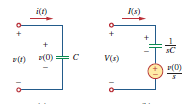
\includegraphics[width=0.8\linewidth]{202/figure/laplace_cap.png}
    \caption{capacitor from time to laplace}
    \label{fig:lap_cap}
\end{figure}

\begin{figure}[H]
    \centering
    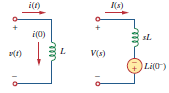
\includegraphics[width=0.8\linewidth]{202/figure/laplace_ind.png}
    \caption{inductor from time to laplace}
    \label{fig:lap_ind}
\end{figure}

\subsection{Phasor}
\begin{defin}
Complex number representation of a sinusoid using amplitude and phase. $v(t) = V_m \cos(\omega t + \phi) = V = V_m \angle \phi$ \\
\begin{itemize}[noitemsep,nolistsep]
    \item $V_m > 0$
    \item $-180^{\circ} < \phi < 180^{\circ}$
    \item $\sin(x+90) = \cos(x)$
    \item \textbf{leading}: In counter clockwise direction positively greater on the complex plane. Else \textbf{lagging}.
\end{itemize}
\end{defin}

% \begin{align*}
%     Z &= A e^{\imath\omega z} 
%     \\ &= A\cos(\omega t + \phi_1) + \imath A\sin(\omega t + \phi_2) 
%     \\ &= A\cos(\omega t + \phi_1) + A_1cos(\omega t + \phi_3) 
%     \\ & = A \angle \phi_1 + A_1 \angle \phi_3 \\
% \end{align*}

\subsubsection{Operations}
$A \angle \Phi_1 \cdot B \angle \Phi_2 = (AB) \angle (\Phi_1 + \Phi_2)$

\begin{question} \mbox{} \\
\begin{itemize}[noitemsep,nolistsep]
    \item Basic complex number calculations.
    \item Use phasor to solve AC circuits: given operating frequency, ask for the value of components.
    \item Find Thevenin equivalent circuit
    \item Superposition of inputs in different frequency.\todo{ASN 3}  
\end{itemize}
\end{question}

\begin{method}
\begin{figure}[H]
    \centering
    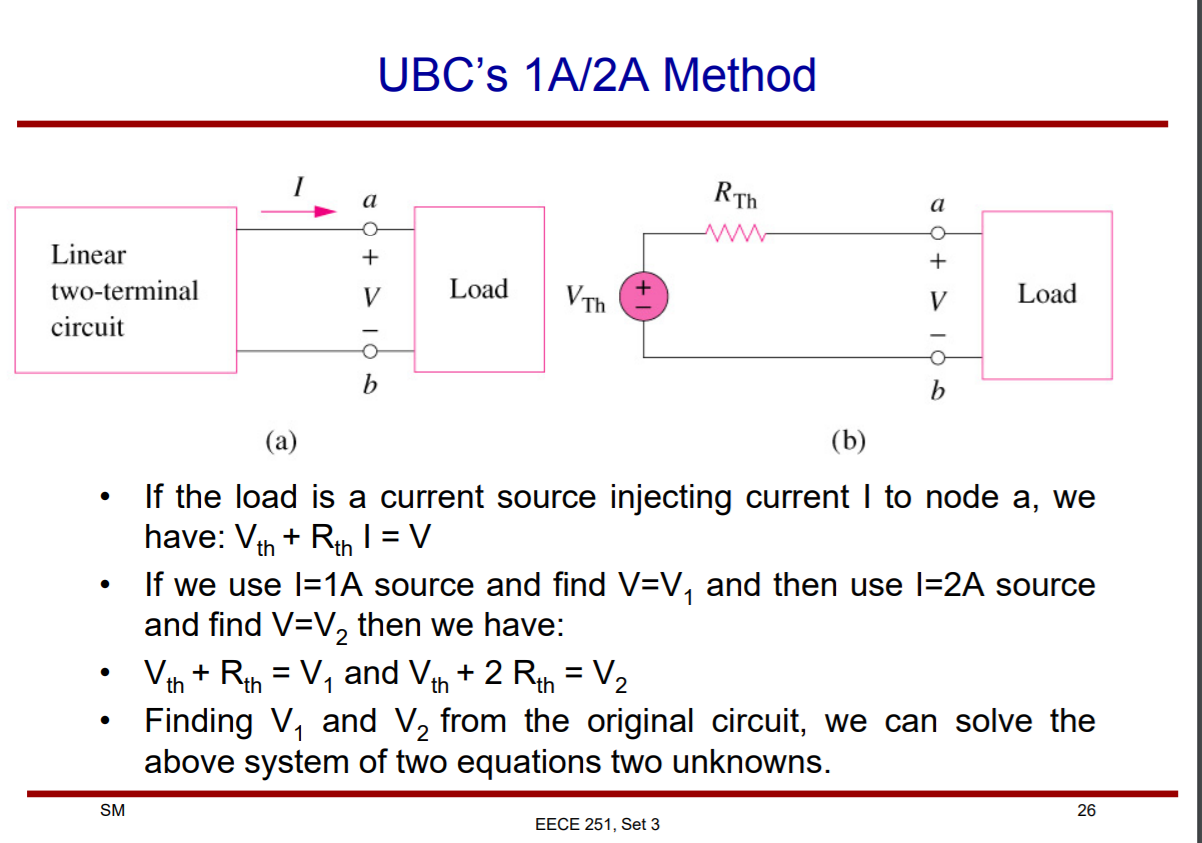
\includegraphics[width=\linewidth]{202/figure/1a_2a.png}
    \caption{\cite{251}}
    \label{fig:1a_2a}
\end{figure}

\textbf{1A/2A method: }
\begin{itemize}[noitemsep,nolistsep]
    \item Replace load with 1A/2A current source. 
    \item Find $V_{1A}$, $V_{2A}$.
    \item Solve $V_{th}$, $R_{th}$ with 
    $\begin{cases}
    V_{th} + R_{th} = V_{1A}\\
    V_{th} + 2R_{th} = V_{2A}\\
    \end{cases}$
\end{itemize}
\end{method}

%%%%%%%%%%%%%%%%%%%%%%%%%%%%%%%%%%%%%%%%%%%%%%%%%%%%%%%%%%%%%
%%%%%%%%%%%%%%%%%%%%%%%%%% section %%%%%%%%%%%%%%%%%%%%%%%%%%
%%%%%%%%%%%%%%%%%%%%%%%%%%%%%%%%%%%%%%%%%%%%%%%%%%%%%%%%%%%%%
\section{Transfer Function}
\begin{defin}
H(s), or transfer function, is the ratio of output response Y(s) to the input excitation X(s), assume the initial condition is zero. \\
\textbf{Stability}: If the transfer function has no pole in the right half-plane, it's stable. 
\end{defin}


\subsection{Bode Plot Elements}
\begin{defin}
\textbf{Unit of decibel(dB)}, For the power gain: 
$G_{dB} = 10 \log_{10}(\frac{P_2}{P_1})$.
For voltage and current, $G_{dB} = 20 \log_{10}(\frac{V_2}{V_1})$ \\
\textbf{decade}: an interval between two frequency with a ratio of 10. \\
\textbf{Bode plot}: 2D plot of Magnitude H (dB) and frequency (decade) as z and x axis. Although there is the third y axis from $\sigma$. 
\end{defin}


\subsection{Construct and Analysis of Bode Plot}
% \textbf{Procedure}: \\
% \begin{itemize}[noitemsep,nolistsep]
%     \item \todo{FInish this}
% \end{itemize}

\subsubsection{General Transfer Function} $$H(w) = \frac{K_1s^{\pm 1}(s+z_0)(s+z_1)^1...(s+z_{n_1})^{n_1}(s+z_z)(s + \overline{z_z})...}{K_2(s+p_0)(s+p_1)^1...(s+p_{n_2})^{n_2}(s + p_z)(s + \overline{p_z})...}$$

\begin{itemize}[noitemsep,nolistsep]
    \item real constant: zero of $\frac{K_1}{K_2}$ or pole of $\frac{K_2}{K_1}$
    \item real simple: zero of s or pole of $\frac{1}{s}$. 
    \item real n order: zero of $(s+z_{n_1})$ or pole of $(s+p_{n_2})^{n_2}$
    \item complex: let $\zeta = \cos\Omega$, where $\Omega= 180^{\circ} - \theta$. Then $p_z = a + \imath b = \omega_0 e^{\imath\Omega}$. Keep in mind that nit all $s^2 + as + b$ are complex.  \\
    $(s + p_z)(s + \overline{p_z})|_{p_z = a + \imath b} = (s^2 + 2\zeta \omega_0 s + \omega_0^2)|_{s=jw} = (\omega_0^2 - \omega^2) + \imath 2 \zeta \omega\omega_0$, which $\approx 40\log_10\omega_0$ when $\omega \ll \omega_0$ and  $\approx 40\log_10\omega$ when $\omega \gg \omega_0$. At around $\omega_0$, $H_{dB} \approx 20\log_{10}(\sqrt{2}) \approx 3$
\end{itemize}

\begin{figure}[H]
    \centering
    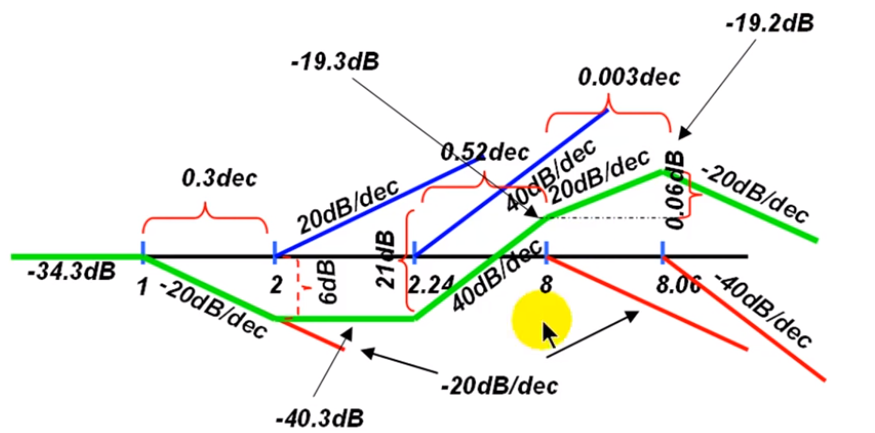
\includegraphics[width=\linewidth]{202/figure/bode_1.png}
    \caption{}
    \label{fig:bode_1}
\end{figure}
zeros create a positive gain, where constant is a positive vertical shift of $20\log_{10}K$, real simple is a ramp with $20N dB/decade$ gain that intersect $\omega$ axis at 1 and real n order is a unit step ramp with $20N dB/decade$ gain that starts at $\omega$, and complex zero has with $40N dB/decade$ gain instead.  \\
poles has negative gain instead of positive. \\


\subsubsection{Phase Plot}
Phase plot has degree/dec as y/x axis.
Zeros create a -45 degree/dec decline, starting from $0.1\omega_0$ to $10\omega_0$, result in a 90 degree decline. no order zero has -45 N degree/dec decline, result in 90 N degree decline. Complex zero is also centered at $\omega_0$, differ in having $\omega_1 = \frac{\omega_0}{10^{\zeta}}$ and $\omega_1 =10^{\zeta} \omega_0$, adn slope of $-\frac{90}{\zeta}$ degree/dec.

\begin{figure}[H]
    \centering
    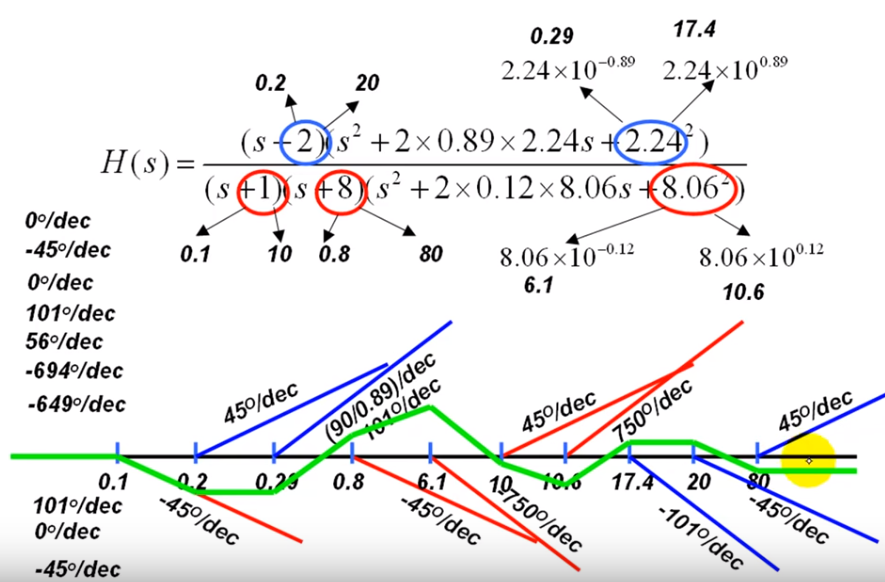
\includegraphics[width=\linewidth]{202/figure/bode_2.png}
    \caption{}
    \label{fig:bode_2}
\end{figure}

% \textbf{Procedure}: \\
% \begin{itemize}[noitemsep,nolistsep]
%     \item find the knees of each pole and zero. 
%     \item \todo{Finish this}
% \end{itemize}

\todo{Plot Bode plot on HP Prime}

\begin{question} \mbox{}\\
\todo{ASN4, 5}\\
\textbf{Transfer function}
\begin{itemize}[noitemsep,nolistsep]
    \item Construct Transfer function from circuit. 
    \item Given Transfer function, ask for the value of each components.
\end{itemize}

\textbf{Bode Plot}
\begin{itemize}[noitemsep,nolistsep]
    \item Approx vs Actual: use Bode plot to approx, use transfer function to calculate the actual values.  
    \item Given a transfer function, plot the Bode plot and Phase plot. 
\end{itemize}
\end{question}

%%%%%%%%%%%%%%%%%%%%%%%%%%%%%%%%%%%%%%%%%%%%%%%%%%%%%%%%%%%%%
%%%%%%%%%%%%%%%%%%%%%%%%%% section %%%%%%%%%%%%%%%%%%%%%%%%%%
%%%%%%%%%%%%%%%%%%%%%%%%%%%%%%%%%%%%%%%%%%%%%%%%%%%%%%%%%%%%%
\section{Filters}
\begin{defin} \mbox{} \\
A filter is a circuit that is designed to pass signals with desired frequencies and reject or attenuate others. \\
\end{defin}

\textbf{Terminologies}: 
In an RLC AC circuit, 
\begin{itemize}[noitemsep,nolistsep]
    \item \textbf{Resonance Frequency}: $$\omega_0 = \frac{1}{\sqrt{LC}}\:rad/s$$ At $\omega_0$, result in purely resisitve circuit with no power loss. Resonance circuit is designed to operate at or near resonant frequency. 
    \item \textbf{Half power frequency}: \\
    $$\omega_{1,2} = \pm \frac{R}{2L} + \sqrt{(\frac{R}{2L})^2 + \frac{1}{LC}}$$, and $\omega_0 = \sqrt{\omega_1\omega_2}$
    \item \textbf{Bandwidth} $B = \omega_2 - \omega_1 = \frac{\omega_0}{Q}$
    \item \textbf{Quality Factor}: ration of resonant frequency to its bandwidth. $$Q = 2\pi \frac{\text{Peak energy stored}}{\text{Energy dissipated in one cycle}}$$ 
    \todo{Q is different for series and parallel circuit}: 
    Series: $Q = \frac{\omega_0L}{R}$, Parallel: $Q = \frac{R}{\omega_0 L}$
    \item for \textbf{high-Q} circuit with $Q \geq 10$, $\omega_{1,2} \approx \omega_0 \pm \frac{B}{2}$
    \item \textbf{Error}: at cutoff frequency, if it's a simple pole/zero, the error is 3dB. 
\end{itemize}

\begin{figure}[H]
    \centering
    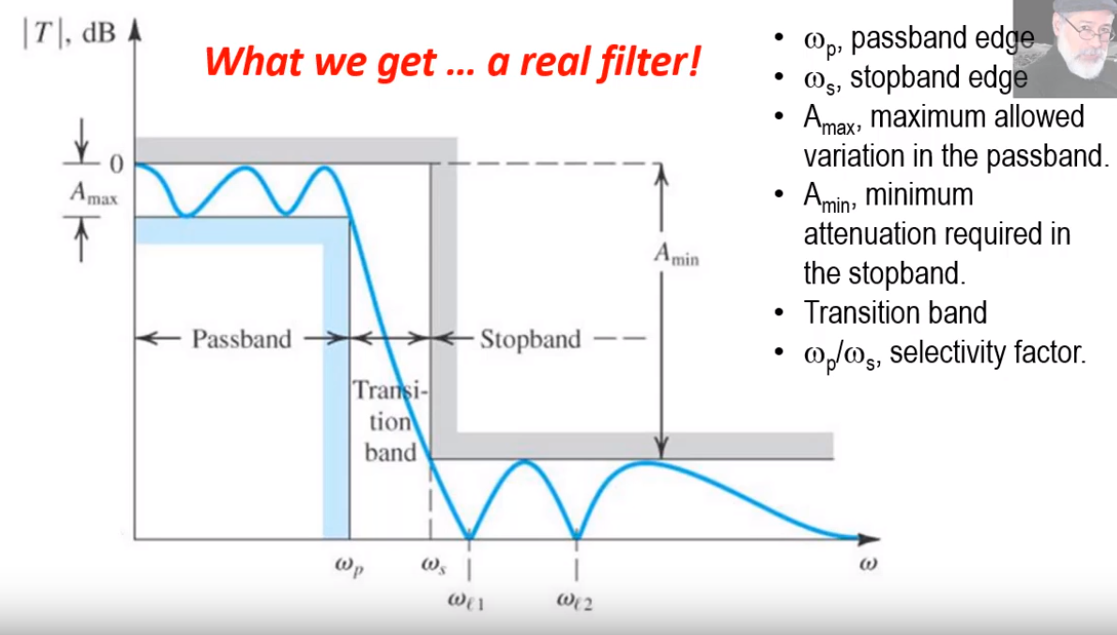
\includegraphics[width=\linewidth]{202/figure/real_filter.png}
    \caption{Elements of real filter}
    \label{fig:real_filter}
\end{figure}


\textbf{Active vs Passive Filters}: 
% Please add the following required packages to your document preamble:
% \usepackage{graphicx}
\begin{table}[H]
\centering
\resizebox{0.6\linewidth}{!}{%
\begin{tabular}{|l|l|}
\hline
type    & adv \& disadv                                                                                          \\ \hline
active  & \begin{tabular}[c]{@{}l@{}}can amp the input\\ not affected by loads\\ dont need inductor\end{tabular} \\ \hline
        & \begin{tabular}[c]{@{}l@{}}less stable\\ not good at high freq\end{tabular}                            \\ \hline
passive & \begin{tabular}[c]{@{}l@{}}stable \\ can have high freq\end{tabular}                                 \\ \hline
        & \begin{tabular}[c]{@{}l@{}}Might have large C, L\\ \\ need tp check cut off freq\end{tabular}          \\ \hline
\end{tabular}%
}
\end{table}

\subsection{Passive Filter}
\begin{itemize}[noitemsep,nolistsep]
    \item High and Low Pass: cutoff frequency(half power, corner) $w_c = \frac{1}{RC}$, or $w_c$ such that $|H(w_c)| = \frac{1}{\sqrt{2}}$
    \item Band Pass
    \item Band Stop
\end{itemize}

\begin{question} \mbox{} \\
\begin{itemize}[noitemsep,nolistsep]
    \item Given components, find the cutoff/corner frequency, or the band corners. \todo{ASN6}
    \item Determine type of filter. 
    \item given frequency and band, find the value of components. 
\end{itemize}
\end{question}

\subsection{Active Filter}
\begin{itemize}[noitemsep,nolistsep]
    \item First Order Low Pass
    \begin{figure}[H]
    \centering
    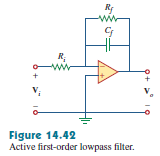
\includegraphics[width=0.6\linewidth]{202/figure/filter_active_lowpass.png}
    \caption{}
    \label{fig:filter_alp}
\end{figure}

    \item First Order High Pass
    \begin{figure}[H]
    \centering
    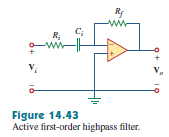
\includegraphics[width=0.6\linewidth]{202/figure/filter_active_highpass.png}
    \caption{}
    \label{fig:filter_ahp}
\end{figure}

    \item Band Pass
    Lower Pass $\rightarrow$ High Pass $\rightarrow$ Inverter
    \begin{figure}[H]
    \centering
    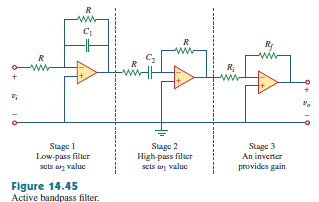
\includegraphics[width=0.8\linewidth]{202/figure/filter_active_bp.png}
    \caption{}
    \label{fig:filter_abp}
\end{figure}

    \item Band reject
    Lower Pass and Highpass $\rightarrow$ Summing opamp. 
    \begin{figure}[H]
    \centering
    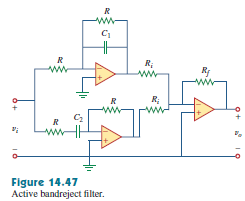
\includegraphics[width=0.8\linewidth]{202/figure/filter_active_br.png}
    \caption{}
    \label{fig:filter_abr}
    \end{figure}
\end{itemize}

\begin{question}\mbox{} \\
\begin{itemize}[noitemsep,nolistsep]
    \item Design a (type of function) filter with pass frequency between x and y Hz, with K(gain) of z
    \item Given a filter configuration, ask for the value of some components in order to archive certain affects. 
    \item \todo{Midterm 3}: given a filter network, as for passband, frequencies, component values. 
\end{itemize}
\end{question}

\subsection{Scaling}
\begin{defin}
Obtain the desired value of an unknown filter from a know filter (usually taking the elementary value of $1\Omega,\; 1H, \; 1F$).
\end{defin}
\textbf{Magnitude Scaling}: \\
Process of increasing all impedance in a network by a factor, the frequency response remaining unchanged

\textbf{Impedance Scaling}: \\
Process of shifting the frequency response of a network up or down the frequency axis while leaving the impedance the same. 

\subsubsection{Scaling Calculation}
Let $K_m$ be the magnitude scaling, $K_f$ be the frequency scaling. 

$$R' = K_m R, \; L' = \frac{K_m}{K_f}L $$
$$C'=\frac{C}{K_mK_f}, \; \omega' = K_f \omega$$
\todo{On webwork, all filters related to scaling are in its \textbf{canonical form}, where $\omega = 1$ rad/s}

\subsection{Advanced Filter Configurations}

\subsubsection{Chebyshev filter}
\begin{defin}
 It's an analog or digital filters having a steeper roll-off and more passband ripple (type I) or stopband ripple (type II) than Butterworth filters. Chebyshev filters have the property that they minimize the error between the idealized and the actual filter characteristic over the range of the filter but with ripples in the passband. 
\end{defin}

\subsubsection{Sallen Key configuration}
\begin{figure}[H]
\centering
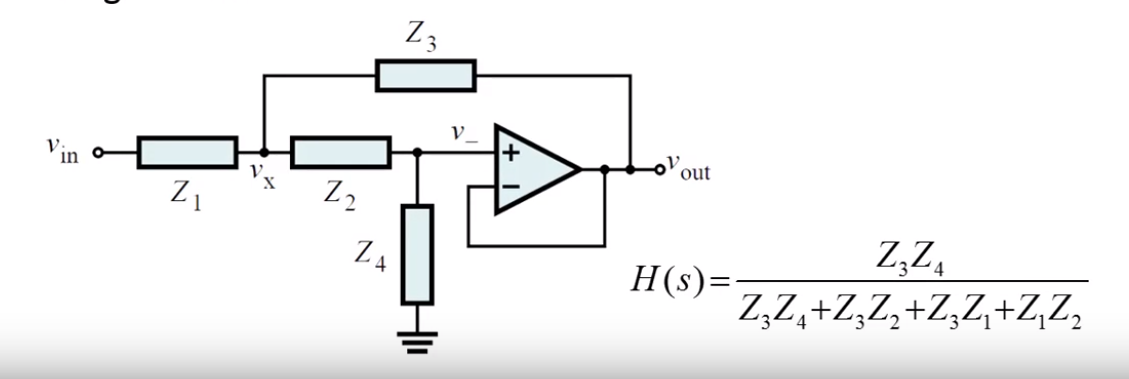
\includegraphics[width=\linewidth]{202/figure/sallen_key_filter.png}
\caption{}
\label{fig:General Sallen Key Filter}
\end{figure}

\subsubsection{Butterworth low pass filter}
\begin{defin}
 A type of signal processing filter designed to have a frequency response as flat as possible in the passband.
\end{defin}


%%%%%%%%%%%%%%%%%%%%%%%%%%%%%%%%%%%%%%%%%%%%%%%%%%%%%%%%%%%%%
%%%%%%%%%%%%%%%%%%%%%%%%%% section %%%%%%%%%%%%%%%%%%%%%%%%%%
%%%%%%%%%%%%%%%%%%%%%%%%%%%%%%%%%%%%%%%%%%%%%%%%%%%%%%%%%%%%%
\section{Two Ports network}
\begin{defin}
Two port network is an electrical network with two separate ports for input and output.
\end{defin}

\begin{figure}[H]
\centering
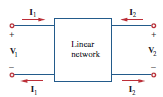
\includegraphics[width=0.5\linewidth]{202/figure/two_port_1.png}
\caption{}
\label{fig:two_port_1}
\end{figure}

\textbf{Most basic form}: \\
$$
\begin{cases}
V_1 = z_{11}I_1 + z_{12}I_2 = \frac{V_1}{I_1}I_1 +  \frac{V_2}{I_1}I_2\\
V_2 = z_{21}I_1 + z_{22}I_2= \frac{V_1}{I_2}I_1 +  \frac{V_2}{I_2}I_2
\end{cases} 
$$ \\ 

$$
\begin{bmatrix}
     V_1 \\
     V_2 
\end{bmatrix}
=
\begin{bmatrix}
    z
\end{bmatrix}
\begin{bmatrix}
     I_1 \\
     I_2 
\end{bmatrix}$$ \\

\subsection{Calculate impedance parameter (z)}
\textbf{Method 1}: add an voltage source to input of the network to get $z_{11}, z_{12}$, and do the same for the output. \\
\textbf{Method 2}: KCL, KVL. 

\subsection{Conversion of two port parameters}
z: impedence parameter \\
y: admittence parameter \\
t: transmission \\ 
Search up the conversion from figure \ref{fig:two_port}
% \todo{Finish this after doing some practices}

%%%%%%%%%%%%%%%%%%%%%%%%%%%%%%%%%%%%%%%%%%%%%%%%%%%%%%%%%%%%%
%%%%%%%%%%%%%%%%%%%%%%%%%% section %%%%%%%%%%%%%%%%%%%%%%%%%%
%%%%%%%%%%%%%%%%%%%%%%%%%%%%%%%%%%%%%%%%%%%%%%%%%%%%%%%%%%%%%
\section{Power}
\begin{defin}
Rate of absorbing or releasing energy. As a convention, absorbing is positive and supplying is negative. 
\end{defin}

\textbf{Instantaneous power(W)}: 
$$p(t) = \frac{1}{2}V_m I_m\cos(\theta_v-\theta_i) + \frac{1}{2} V_m I_m \cos(2\omega t + \theta_v + \theta_i)$$ \\

\textbf{Average power(W)}:
$$P = \frac{1}{2}V_m I_m\cos(\theta_v-\theta_i)$$ \\

\textbf{Complex power(VA)}:
\begin{equation*}
    \begin{aligned}
        \pmb{S} & = \frac{1}{2} \pmb{V}\pmb{I}^{*} \\
    & =\pmb{V_{rms}}\pmb{I_{rms}}^{*}  \\
    & = V_{rms}I_{rms} \angle (\theta_v - \theta_i) \\
    & = P + \imath Q \\
    \end{aligned}
\end{equation*}

\textbf{Apparent power(VA)}:
\begin{equation*}
\begin{aligned}
    S  & = |\pmb{S}| \\
     & = V_{rms} I_{rms} = \frac{1}{2} V_m I_m \\
     & = \sqrt{P^2 + Q^2} \\
\end{aligned}
\end{equation*}

\textbf{Power factor}:\\
pf lag: I lags or V leads I \\
pf lead: I leads or V lags I \\
$$pf = \frac{P}{S} = \cos(\theta_v - \theta_i)$$ 

\textbf{Real power(W)}
$$P = \Re(\pmb{S}) = S\cos(\theta_v - \theta_i)$$

\textbf{Reactive power(VAR)}
$$Q = \Im(\pmb{S}) = S\sin(\theta_v - \theta_i)$$



\subsection{Three Phase System}

\begin{defin}
A system produced by a generator consisting of three sources having the same amplitude and frequency but out of phase with each other by $120^{\circ}$.
\end{defin}

\subsubsection{Balanced three phase}

\textbf{Balanced voltage}: source voltage are equal in magnitude.  \\
\textbf{Balanced load}: phase impedance are equal in magnitude and phase. \\
\textbf{Line voltage}: voltage from line x to line y.  \\
\textbf{Phase voltage}: voltage from line to neutral line \\
\textbf{Line current}: current in the line, from source(usually left) to right.  \\
\textbf{Phase current}: current of each phase or source or load. \\



\textbf{Connection types}
\begin{itemize}[noitemsep,nolistsep]
    \item $Y - Y$: \\
    Provided $V_p$: \\
    Phase voltage: $
    \begin{cases}
    V_{an} = V_p \angle 0^{\circ} \\
    V_{bn} = V_p \angle -120^{\circ} \\
    V_{cn} = V_p \angle 120^{\circ}   
    \end{cases}
    $\\
    
    Line voltage:$
    \begin{cases}
    V_{ab} = V_{an} - V_{bn} = \sqrt{3} V_p \angle 30^{\circ} \\
    V_{bc} = V_{bn} - V_{cn} = \sqrt{3} V_p \angle -90^{\circ} \\
    V_{ca} = V_{cn} - V_{an} = \sqrt{3} V_p \angle 150^{\circ} 
    \end{cases}
    $
    
    Line current:$
    \begin{cases}
    I_{a} = \frac{V_{an}}{Z_Y} \\
    I_{b} =I_a \angle -120^{\circ} \\
    I_{c} = I_a \angle 120^{\circ}
    \end{cases}
    $
    

\begin{figure}[H]
    \centering
    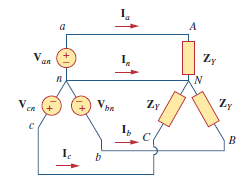
\includegraphics[width=0.5\linewidth]{202/figure/y-y.png}
    \caption{}
    \label{fig:y-y}
\end{figure}

    \item $\Delta - \Delta$ \\
Since each load and source are parallel, the phase current can be calculated, and then line current.
    
\begin{figure}[H]
    \centering
    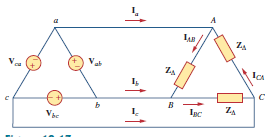
\includegraphics[width=0.5\linewidth]{202/figure/d-d.png}
    \caption{}
    \label{fig:d-d}
\end{figure}

    \item $Y - \Delta$ \\
    Change the $\Delta$ configuration to Y by : \\
    $
    \begin{cases}
    Z_{\Delta} = 3Z_Y \\
    Z_Y = \frac{Z_{\Delta}}{3}
    \end{cases}
    $
    
    
\begin{figure}[H]
    \centering
    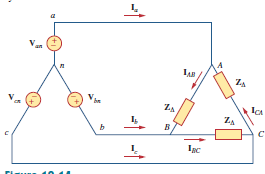
\includegraphics[width=0.5\linewidth]{202/figure/y-d.png}
    \caption{}
    \label{fig:y-d}
\end{figure}

    \item $\Delta - Y$: \\

\begin{figure}[H]
    \centering
    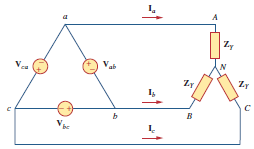
\includegraphics[width=0.5\linewidth]{202/figure/d-y.png}
    \caption{}
    \label{fig:d-y}
\end{figure}

    Change $\Delta$ to Y: First find $V_L$ with the phase voltage of $\Delta$, then get the line voltage for Y configuration.  
    
\begin{figure}[H]
    \centering
    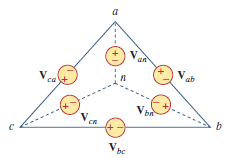
\includegraphics[width=0.5\linewidth]{202/figure/d_source_to_y.png}
    \caption{}
    \label{fig:ds_2_y}
\end{figure}

   Phase voltage: $
    \begin{cases}
    V_{ab} = V_L \angle 0^{\circ} \\
    V_{bc} = V_L \angle -120^{\circ} \\
    V_{ca} = V_L \angle 120^{\circ}   
    \end{cases}
    $\\
    
    Line voltage: $
    \begin{cases}
    V_{an} =\frac{1}{\sqrt{3}} V_L \angle -30^{\circ} \\
    V_{bn} =\frac{1}{\sqrt{3}} V_L \angle -150^{\circ} \\
    V_{cn} =\frac{1}{\sqrt{3}} V_L \angle 90^{\circ} \\
    \end{cases}
    $
\end{itemize}

\textbf{Power of Three Phase}: \\
For Y configuration: 
$\begin{cases}
I_p = I_L \\
\sqrt{3} V_p = V_L
\end{cases}$
\\
For $\Delta$ configuration: 
$\begin{cases}
\sqrt{3} I_p = I_L \\
V_p = V_L
\end{cases}$
\begin{itemize}[noitemsep,nolistsep]
    \item Average Power: $3P = 3V_pI_P\cos(\theta_v-\theta_i) =  \sqrt{3}V_LI_L\cos(\theta_v-\theta_i)$
    \item Reactive Power: $3Q =3V_pI_P\sin(\theta_v-\theta_i) = \sqrt{3}V_LI_L\sin(\theta_v-\theta_i)$
    \item Apparent Power: $3S =3V_pI_P = \sqrt{3}V_LI_L$
    \item Complex Power: $3\pmb{S} =3V_pI_p \angle\theta \sqrt{3}V_LI_L\angle\theta$
\end{itemize}
\todo{power loss in three phase.}

\subsubsection{Unbalanced three phase}
Since $I_n$ is no longer 0, take that into account. 

\begin{question}
Given a three phase system, provides it's complex power and ask for line current, voltage. Ask for ways to raise power factor to unity. 
\end{question}

%%%%%%%%%%%%%%%%%%%%%%%%%%%%%%%%%%%%%%%%%%%%%%%%%%%%%%%%%%%%%
%%%%%%%%%%%%%%%%%%%%%%%%%% section %%%%%%%%%%%%%%%%%%%%%%%%%%
%%%%%%%%%%%%%%%%%%%%%%%%%%%%%%%%%%%%%%%%%%%%%%%%%%%%%%%%%%%%%
\section{Transformer}
There are in total 4 configuration types for parallel coil, two for series. See figure \ref{fig:trans_series}, $L_{total} = L_1 + L2 + 2M$. In the other case of series,  $L_{total} = L_1 + L2 - 2M$

\begin{figure}[H]
    \centering
    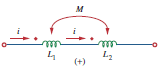
\includegraphics[width=0.5\linewidth]{202/figure/transformer_2_a.png}
    \caption{}
    \label{fig:trans_series}
\end{figure}

\textbf{Dot Convention}: \\
if a current enters the doted terminal of one coil, the reference polarity of the mutual voltage in the second coil is positive at the dotted terminal of the second coil.

\begin{question}
Given circuit components of a transformer circuit, ask for phasor current or impedance of one side, or any missing circuit components. 
\end{question}

\begin{method}
See figure \ref{fig:trans_simplification} to simply the circuit, then use KCL to solve. \todo{Be careful with the direction of current!}
\end{method}

\begin{figure}[H]
    \centering
    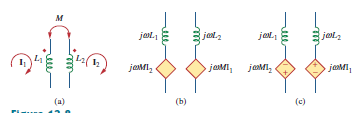
\includegraphics[width=\linewidth]{202/figure/transformer_1.png}
    \caption{}
    \label{fig:trans_simplification}
\end{figure}


\subsection{Energy In Transformer}
\begin{defin}
\textbf{Instantaneous energy stored:}\\
\begin{equation} \label{eq:energy}
  w = \frac{1}{2}L_1I^2_1 + \frac{1}{2}L_2I^2_2 \pm M i_1i_2  
\end{equation}

where the $\pm$ is determined by if both current enter or leave dot. \\
\textbf{Coupling coefficient: }
$k = \frac{M}{\sqrt{L_1L_2}} \; 0 \leq k \leq 1$, measure of magnetic coupling between two coils, if $k  > 0.5$, they are tightly coupled, else loosely. \\
\end{defin}

\begin{question}
Calculate energy in circuit at given time of a time domain voltage input. 
\end{question}
\begin{method}
Just plug \ref{eq:energy} into the circuit after all circuit components are calculated. Use $\pmb{S} = \pmb{V}\pmb{I^{*}}$ for power in each components. 
\end{method}


\subsection{Ideal Transformer}
\begin{defin}
Transformer circuit with the following assumption: \\
\begin{itemize}[noitemsep,nolistsep]
    \item large reactants: $L_1,L_2,M \rightarrow \infty$
    \item coupling coefficient equals to unity, $k=1$
    \item both oils are lossless ($R_1 = R_2 = 0$)
    \item $Z_{in} = \frac{Z_L}{n^2}$ to calculate how load impedance reflects to the primary side. 
    \item With these assumptions, we can say use turn ratio $n = \frac{N_2}{N1} = \frac{V_2}{V_1} = \frac{I_1}{I_2}$. 
\end{itemize}

\end{defin}

\begin{question}
Given circuit components of a transformer circuit, ask for phasor current or impedance of one side, or any missing circuit components. 
\end{question}

\begin{method} \mbox{} \\
\begin{enumerate}[noitemsep,nolistsep]
    \item See figure \ref{fig:trans_ideal_simp} to simply the circuit, then use KCL to solve.
    \item Assign current and voltage to each coil, use turn ratio to complete KVL/KCL to solve the circuit. 
\end{enumerate}
\end{method}

\begin{figure}[H]
    \centering
    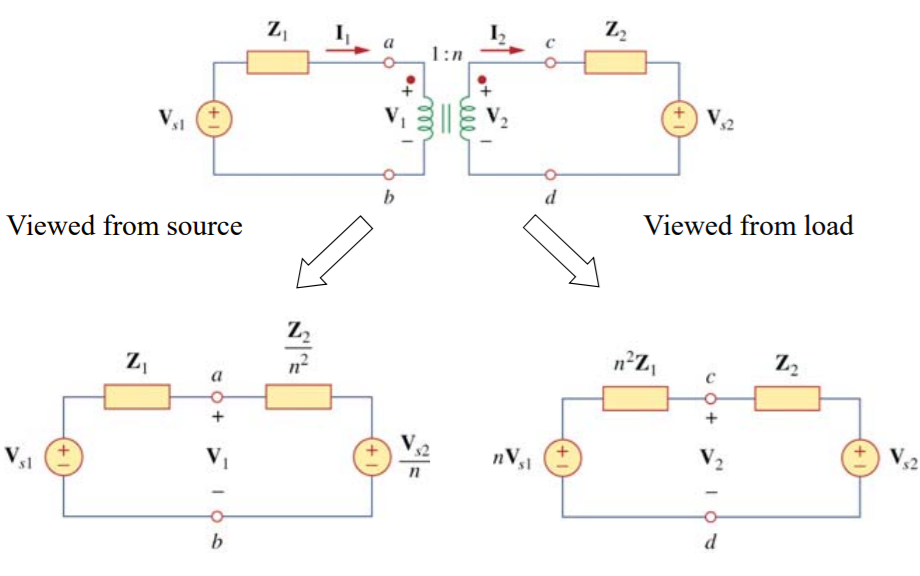
\includegraphics[width=0.9\linewidth]{202/figure/trrans_3.png}
    \caption{}
    \label{fig:trans_ideal_simp}
\end{figure}


%%%%%%%%%%%%%%%%%%%%%%%%%%%%%%%%%%%%%%%%%%%%%%%%%%%%%%%%%%%%%
%%%%%%%%%%%%%%%%%%%%%%%%%% section %%%%%%%%%%%%%%%%%%%%%%%%%%
%%%%%%%%%%%%%%%%%%%%%%%%%%%%%%%%%%%%%%%%%%%%%%%%%%%%%%%%%%%%%
\section{Second Order Circuit}
\begin{defin}
Any circuits that can be simplify to a second order ODE. 
\end{defin}
\begin{figure}[H]
    \centering
    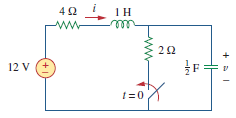
\includegraphics[width=0.5\linewidth]{202/figure/soc_general.png}
    \caption{Example of Second Order Circuit 2}
    \label{fig:soc_1}
\end{figure}
\begin{figure}[H]
    \centering
    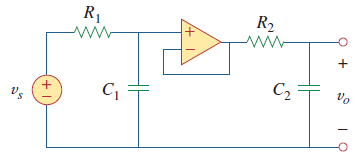
\includegraphics[width=0.5\linewidth]{202/figure/soc_opamp.png}
    \caption{Example of Second Order Circuit 2}
    \label{fig:soc_2}
\end{figure}

\subsection{Source-Free}
\begin{defin}
Any Second order circuits without any independent source. It's steady state will include a steady state inductor and/or capacitor.
\end{defin}

\textbf{Solve Source-Free}:\\ 
\textbf{damping factor}: $\alpha = \frac{\mathrm{L}}{\mathrm{2R}}$ \\
\textbf{resonance frequency}: $\omega_0 = \frac{1}{\sqrt{LC}}$ \\
After transform a general source free RLC circuit into laplace, solve the characteristic function with $s = -\alpha \pm \sqrt{\alpha^2 + \omega_0^2}$ based on $\Delta = \sqrt{4\alpha^2 - 4w_0^2}$. The eigenvalue gives:
\begin{itemize}[noitemsep,nolistsep]
    \item overdamped: $\alpha > \omega_0$
    \item critically damped: $\alpha = \omega_0$
    \item underdamped: $\alpha < \omega_0$
\end{itemize}

\begin{question}
Given a RLC circuit and $I_0$, $V_0$ of inductor and capacitor, 
\end{question}


\subsection{Step-Response}
\begin{defin}
RLC circuit was introduced instantaneously by a source. Solve for $v(t)$ in RLC series cirucit, $i(t)$ in RLC parallel circuit. 
\end{defin}

\textbf{Solve Step-Response}: 
Let $v_t(t)$ be the transient response, $v_{ss}(t)$ be the steady state response. $v_t(t)$ is the homogeneous solution to RLC circuit, where $v_{ss}(t)$ is the partical solution. 
$\pmb{v(t) = v_t(t) + v_{ss}(t)}$ 

\subsection{General Second Order Circuit}
\begin{method} \mbox{} \\
\begin{itemize}[noitemsep,nolistsep]
    \item determine $x(0^+),\frac{\mathrm{d}x}{\mathrm{d}t}(0^+),x(\infty) $ and other initial conditions for the ODE. 
    \item find $x_t(t)$ by turning off independent source, plug in initial condition and boundary values. \todo{Construct KCL/KVL using function of time, and extract ODE for a value}. Note that KVL is simpler for inductor only circuit, KCL is easier for capacitor. 
    \item $x(t) = x_t(t) + x_{ss}(t)$, where $x_{ss}(t)$ is $x(\infty)$.
\end{itemize}
\end{method}


\begin{question} \mbox{} \\
\begin{itemize}[noitemsep,nolistsep]
    \item Given a circuit, solve for $v_0(t), i_0(t)$: \textbf{ASN13.10, 11}
    \item 
\end{itemize}

\end{question}

    

%%%%%%%%%%%%%%%%%%%%%%%%%%%%%%%%%%%%%%%%%%%%%%%%%%%%%%%%%%%%%
%%%%%%%%%%%%%%%%%%%%%%%%%% section %%%%%%%%%%%%%%%%%%%%%%%%%%
%%%%%%%%%%%%%%%%%%%%%%%%%%%%%%%%%%%%%%%%%%%%%%%%%%%%%%%%%%%%%
\bibliographystyle{unsrt}
\bibliography{202}
\end{multicols}

\newpage
%%%%%%%%%%%%%%%%%%%%%%%%%%%%%%%%%%%%%%%%%%%%%%%%%%%%%%%%%%%%%
%%%%%%%%%%%%%%%%%%%%%%%%%% section %%%%%%%%%%%%%%%%%%%%%%%%%%
%%%%%%%%%%%%%%%%%%%%%%%%%%%%%%%%%%%%%%%%%%%%%%%%%%%%%%%%%%%%%
\section{HP Primer a Primer}

HUGE TABLE INCOMING

% Please add the following required packages to your document preamble:
% \usepackage{graphicx}
\begin{table}[h]
\centering
% \resizebox{\textwidth}{!}{%
\begin{tabular}{|l|l|l|}
\hline
Command  & Parameter    & Function         \\ \hline
laplace  & (f(t), t, s) &                  \\ \hline
ilaplace & (F(s), s, t) & inverse laplace  \\ \hline
partfrac & (f(x))       & partial fraction \\ \hline
evalf    & (f(x))       &                  \\ \hline
proot    & (f(x))    & get the root of polynoimal                  \\ \hline
normal   &              &                  \\ \hline
solve    &  {system of equations}, {variables}            &                  \\ \hline
fsolve    & same as solve, sometimes              &                  \\ \hline

\end{tabular}%
% }
\end{table}

%%%%%%%%%%%%%%%%%%%%%%%%%%%%%%%%%%%%%%%%%%%%%%%%%%%%%%%%%%%%%
%%%%%%%%%%%%%%%%%%%%%%%%%% section %%%%%%%%%%%%%%%%%%%%%%%%%%
%%%%%%%%%%%%%%%%%%%%%%%%%%%%%%%%%%%%%%%%%%%%%%%%%%%%%%%%%%%%%
\newpage
% \begin{figure*}
%     \centering
%     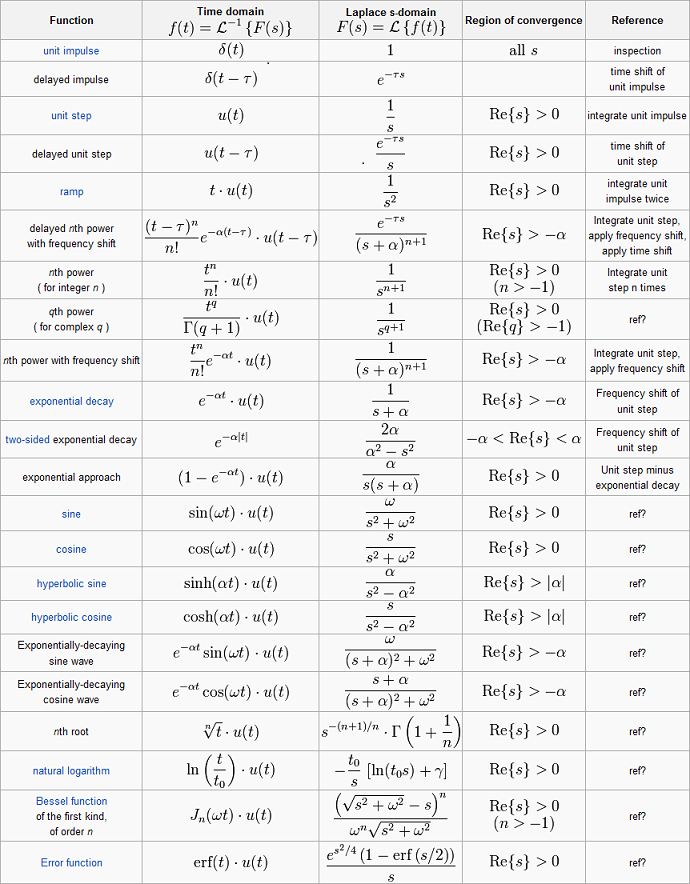
\includegraphics[width=0.8\textwidth,height=\textheight,keepaspectratio]{202/figure/lapace_table.png}
%     \caption{Table of Laplace \cite{oneill}}
%     \label{fig:lapace_tb_1}
% \end{figure*}

% \begin{figure*}
%     \centering
%     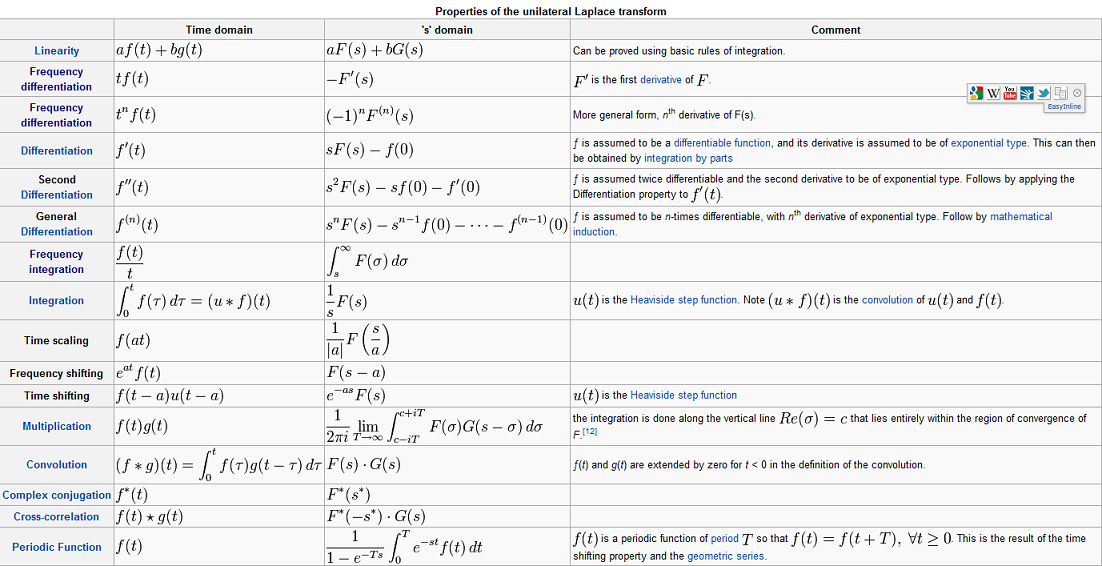
\includegraphics[width=\textwidth,height=\textheight,keepaspectratio]{202/figure/lapace_table_2.png}
%     \caption{Operation of Laplace \cite{oneill}}
%     \label{fig:lapace_tb_2 }
% \end{figure*}

\begin{figure*}
    \centering
    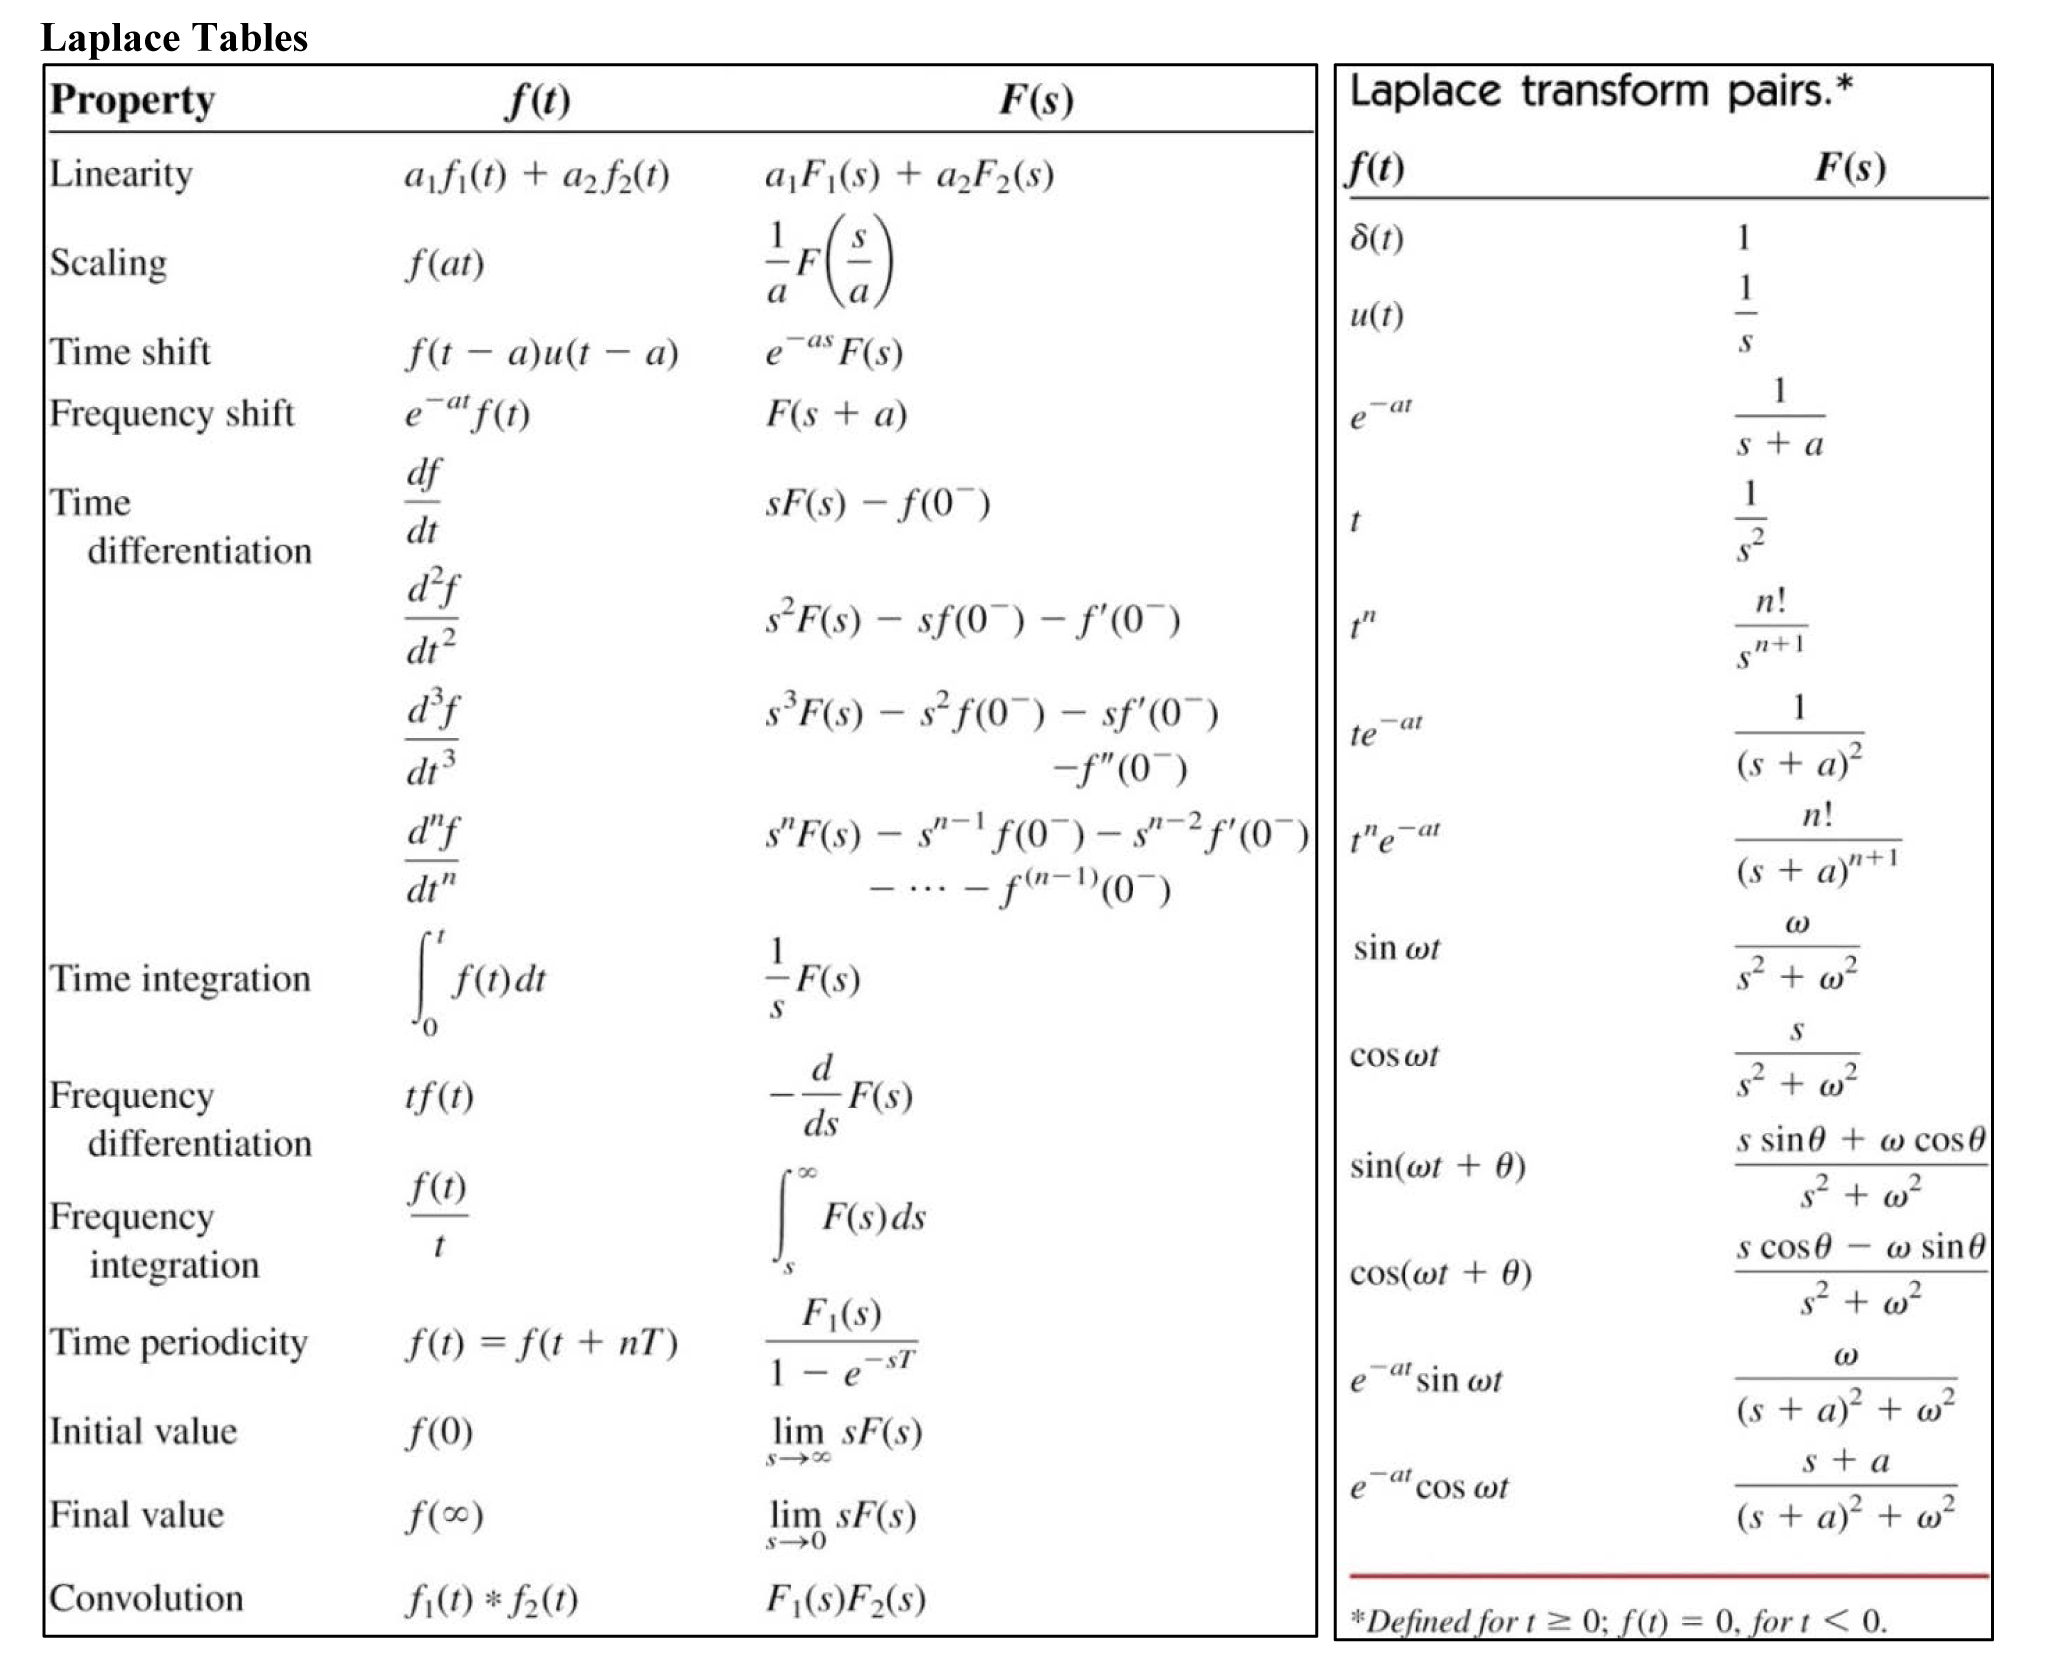
\includegraphics[width=0.8\textwidth,height=\textheight,keepaspectratio]{202/figure/laplace_transforms.png}
    \caption{Table of Laplace \cite{linares}}
    \label{fig:lapace_tb}
\end{figure*}

\begin{figure*}
    \centering
    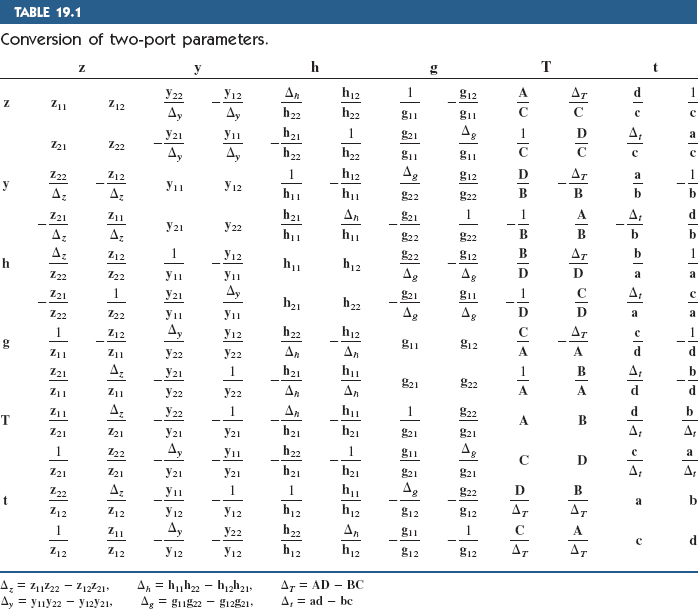
\includegraphics[width=0.8\textwidth,height=\textheight,keepaspectratio]{202/figure/two_port_network_conversion_table.jpg}
    \caption{Two Port Network Conversion Table \cite{linares}}
    \label{fig:two_port}
\end{figure*}
\end{document}
